\documentclass[10pt,twocolumn,letterpaper]{article}

\usepackage{epsfig}
\usepackage{graphicx}
\usepackage{amsmath}
\usepackage{amssymb}
\usepackage[breaklinks=true,bookmarks=false]{hyperref}
\usepackage{float}
\usepackage{caption}
\usepackage{enumitem}
\usepackage{ragged2e} % Added for justification

\def\cvprPaperID{****} % Enter the CVPR Paper ID here
\def\httilde{\mbox{\tt\raisebox{-.5ex}{\symbol{126}}}}

\justifying % Apply global justification

\setcounter{page}{1}

\begin{document}

%%%%%%%%% TITLE
\title{Predictive Analysis of Baccalà Sales: Insights and Challenges for Arte Culinaria da Jhonny}

\author{
Flavio Kaci\\
{\tt\small 2124007}
\and
Antonio Mattesco\\
{\tt\small 2104368}
\and 
Alberto Calabrese\\
{\tt\small 2103405}
}

\date{}
\maketitle


\section{Introduction}

The culinary arts have always played a significant role in Italy’s cultural and economic landscape, with each region contributing to the nation’s rich gastronomic heritage. In Treviso, renowned for its historic charm and vibrant culinary traditions, \textit{Arte Culinaria da Jhonny}, a family-run business based in Mignagola (TV) and owned by Flavio’s uncle, stands out for its artisanal approach to preparing delicacies for local gastronomy shops. Among its offerings, Baccalà has become a hallmark of excellence, driving demand and solidifying the laboratory’s position in the regional culinary scene. This report explores the time series data related to this iconic dish, analyzing production and consumption patterns for a single customer, a gastronomy near Treviso.

The analysis leverages data from \textit{Arte Culinaria da Jhonny}, focusing on the production and supply of Baccalà, which are crucial for optimizing internal processes and ensuring consistent supply to gastronomy shops. By applying advanced statistical techniques and predictive modeling, we aim to identify key \textbf{trends}, \textbf{seasonality}, and \textbf{anomalies}, enabling the laboratory to make informed decisions about inventory management and resource allocation.

Despite the challenges posed by a limited dataset, we have chosen to maintain the authenticity of the real-world data provided by \textit{Arte Culinaria da Jhonny}. Working with a small dataset and with just a few variables underscores the complexity of forecasting in a real operational context, where data scarcity is a common issue, yet accurate predictions remain crucial.

A central goal of this report is to develop a \textbf{short-term forecasting model} and give and provide the laboratory with \textbf{useful and actionable information} on how to improve and which data to monitor in the future. Predictions are vital for balancing supply and demand, especially given the perishable nature of food products and the seasonal fluctuations in the culinary industry.

This analysis aligns with a growing focus on efficiency and resilience in supply chains, particularly in an era of evolving consumer preferences and heightened awareness of food waste.

\section{Data}
\subsection{Data Gathering}
The data analyzed in this report were sourced from the archival records of the \textbf{billing software} utilized by the laboratory. This software has proven instrumental in compiling a comprehensive dataset on Baccalà sales, spanning a period from January $2021$ to December $2024$. The dataset consists of $48$ monthly observations, providing a robust foundation for time-series analysis.

Each observation in the dataset is structured into three columns:
\begin{itemize}
    \item \textbf{Date}: Represents the specific month and year of the recorded sale.
    \item \textbf{Baccalà\_Mantecato}: Indicates the quantity (in kg) of Baccalà Mantecato sold during the corresponding period.
    \item \textbf{Baccalà\_Vicentina}: Indicates the quantity (in kg) of Baccalà alla Vicentina sold during the corresponding period.
\end{itemize}


This dataset offers valuable information on the dynamics of Baccalà production and consumption, allowing the identification of patterns and trends that can inform \textbf{strategic decision making}. By examining these variables over time, we aim to uncover the underlying factors influencing demand and develop predictive models to \textbf{improve operational efficiency}.

\subsection{Data Preprocessing}
To ensure the data was ready for analysis, several \textbf{preprocessing} steps were undertaken. Firstly, the "Date" column was converted into an appropriate date format, allowing for accurate temporal analysis. Additional features such as "\textbf{Month}" and "\textbf{Year}" were derived from the "\textbf{Date}" column to facilitate the identification of seasonal trends and interannual variations. A \textbf{trend} variable was also introduced to capture the temporal progression of the dataset.

Missing values were checked and confirmed to be absent, ensuring the dataset's integrity. Alongside the primary dataset, an external dataset containing information on salmon consumption in Italy was integrated. This dataset, sourced from \href{https://eumofa.eu/first-sale-weekly-data}{EUMOFA}, provided monthly observations on salmon sales, starting from January $2009$. The inclusion of this dataset was motivated by its potential to serve as an \textbf{explanatory variable} in modeling Baccalà sales. 

The salmon dataset included three key variables:
\begin{itemize}
    \item \textbf{Date}: The month and year of salmon consumption, starting from November $2020$. A two-month lag was applied to align with future forecasting scenarios.
    \item \textbf{kg\_std}: The standardized quantity of salmon consumed (in kilograms), used to simplify comparative analysis.
    \item \textbf{kg}: The raw quantity of salmon consumed (in kilograms).
\end{itemize}

These data were aggregated and aligned with the Baccalà dataset to ensure \textbf{temporal consistency} and \textbf{compatibility}. While other external variables, such as the NIC for fish products and production prices sourced from Istat, were initially considered, they were excluded due to their lack of statistical significance or mismatched temporal resolution.

The combined dataset now offers a comprehensive view of Baccalà sales alongside relevant external factors, setting the stage for robust time series analysis and predictive modeling. 

The resulting dataset (Tab.~\ref{table:resulting_dataset}), looks like:
\begin{table}[h!]
\centering
\resizebox{1\linewidth}{!}{%
\begin{tabular}{|l|r|r|r|r|r|r|}
\hline
\textbf{Date} & \textbf{Mant.} & \textbf{Vic.} & \textbf{M.} & \textbf{Y.} & \textbf{Trend} & \textbf{Fish Cons} \\
\hline
2021-01-01 & 36.4 & 6.1 & 01 & 2021 & 1 & 0.8904992 \\
2021-02-01 & 36.4 & 5.4 & 02 & 2021 & 2 & 2.7444439 \\
2021-03-01 & 31.2 & 6.1 & 03 & 2021 & 3 & 0.6030702 \\
\hline
\end{tabular}%
}
\caption{Resulting dataset}
\label{table:resulting_dataset}
\end{table}

\section{Explanatory Analysis}

\begin{figure}[h!]
    \centering
    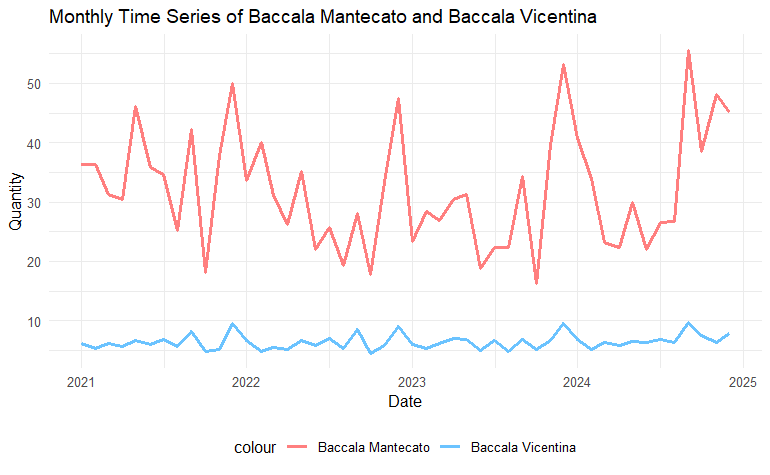
\includegraphics[width=0.5\textwidth]{PlotsBEFD/SS_MAN_VIC.png} 
    \caption{}
    \label{fig:SS_MAN_VIC}
\end{figure}

The exploratory phase of the analysis begins with visualizing the time series data for Baccalà Mantecato and Baccalà Vicentina. This visualization (Fig.~\ref{fig:SS_MAN_VIC}) provides a comparative view of the monthly sales trends for both products. Notably, the sales quantities of Baccalà Mantecato consistently exceed those of Baccalà Vicentina across all observed periods. Furthermore, \textbf{Baccalà Mantecato} demonstrates greater \textbf{variability in sales}, with a wider range of values, while \textbf{Baccalà Vicentina} exhibits a \textbf{more stable pattern}. Both products, however, show a pronounced \textbf{increase in sales} during the final months of each year, particularly in December.

To further explore yearly patterns, separate time series plots grouped by year were created for each product (Fig.~\ref{fig:Month_SS_MAN_VIC}). These plots reveal consistent seasonal trends, with sales peaking in the latter months of the year, particularly in September and December. For Baccalà Mantecato, the data also suggest a shift over time: during the first year ($2021$), sales volumes in off-peak months were generally higher compared to subsequent years, while peak-month sales have increased in recent periods.

\begin{figure}[h!]
    \centering
    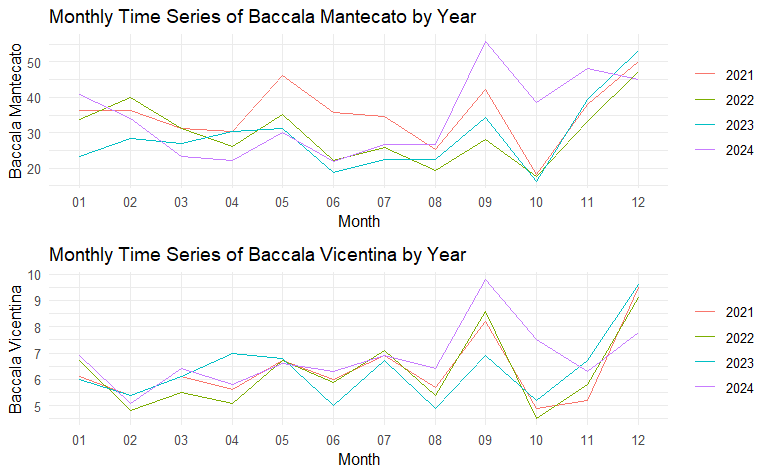
\includegraphics[width=0.5\textwidth]{PlotsBEFD/Month_SS_MAN_VIC.png} 
    \caption{}
    \label{fig:Month_SS_MAN_VIC}
\end{figure}

The \textbf{autocorrelation functions} (ACF) of the time series were analyzed to examine the presence of seasonality and lagged relationships (Fig.~\ref{fig:ACF_MAN}, Fig.~\ref{fig:ACF_VIC}).
\begin{figure}[h!]
    \centering
    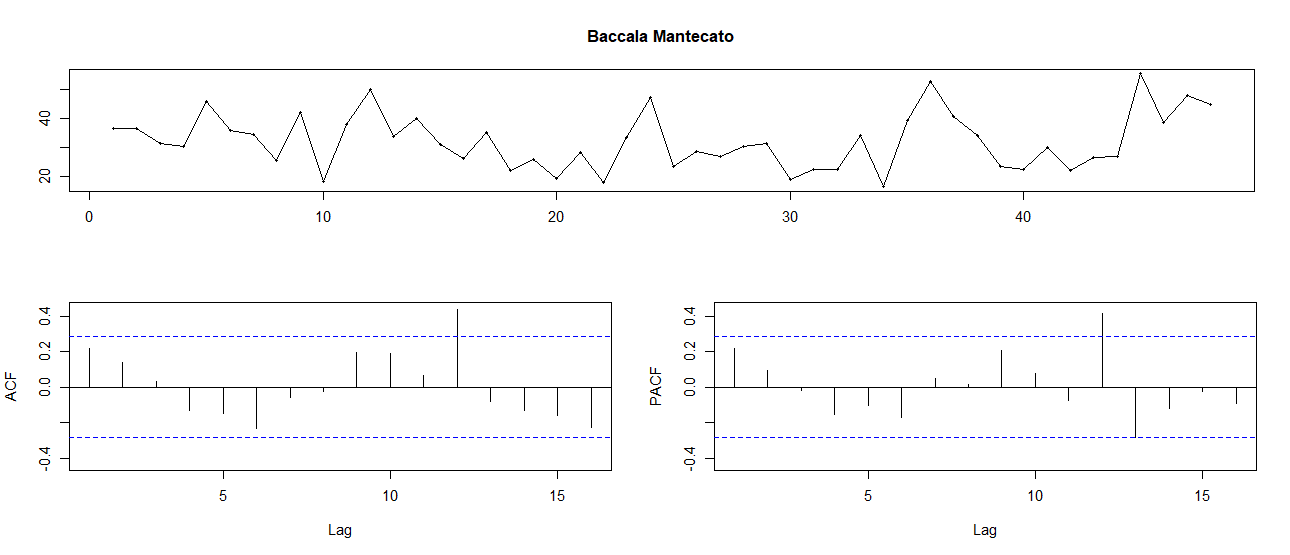
\includegraphics[width=0.5\textwidth]{PlotsBEFD/ACF_MAN.png} 
    \caption{}
    \label{fig:ACF_MAN}
\end{figure}
\begin{figure}[h!]
    \centering
    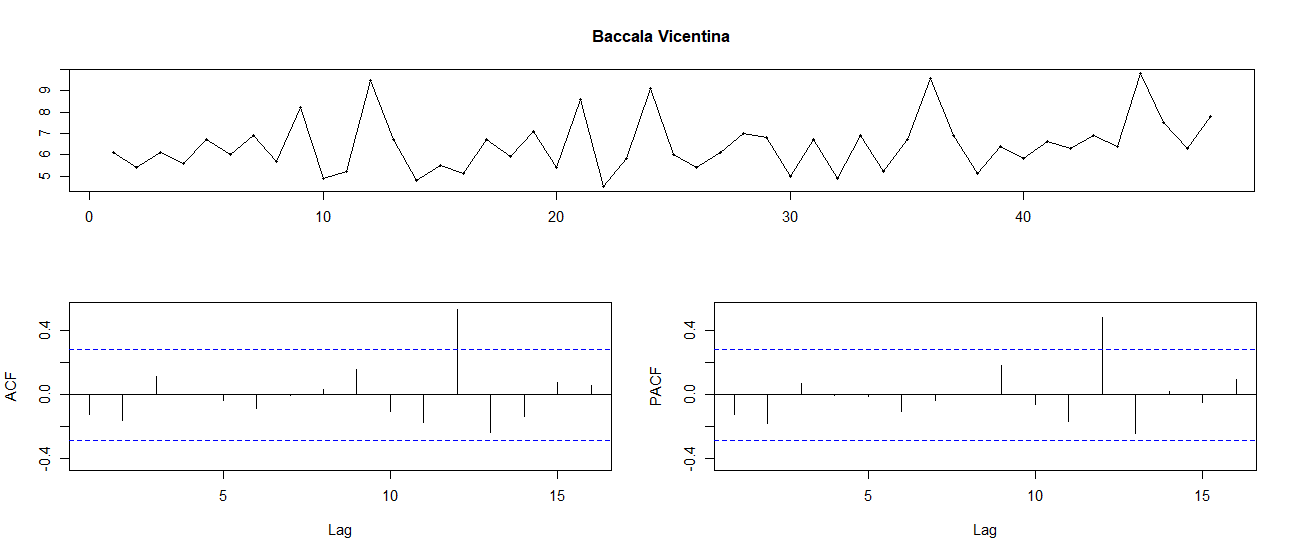
\includegraphics[width=0.5\textwidth]{PlotsBEFD/ACF_VIC.png} 
    \caption{}
    \label{fig:ACF_VIC}
\end{figure}

Most autocorrelations fall within the confidence bands, indicating an absence of significant correlation for most lags. However, the sinusoidal pattern observed within the bands suggests periodic fluctuations, with a notable peak at lag $12$, supporting the hypothesis of \textbf{annual seasonality}. This periodic effect will be further evaluated by analyzing the residuals of future forecasting models to confirm or refute the presence of seasonality.

The insights gained from this exploratory analysis lay the groundwork for constructing robust predictive models that incorporate both seasonal and trend components. These models aim to enhance the laboratory's ability to \textbf{forecast sales} and \textbf{optimize inventory management}, ultimately contributing to its operational efficiency and market responsiveness.

\section{Train-Test Split}
To evaluate the predictive performance of forecasting models, the dataset was divided into \textbf{training} and \textbf{testing} subsets.

The \textbf{training set} includes observations from the initial $80$\% of the time periods, while the \textbf{test set} consists of the final $20$\%. By design, this approach preserves the temporal structure of the data, preventing data leakage and ensuring that predictions are based solely on prior information.

For visualization purposes, the split was applied to both Baccalà Mantecato and Baccalà Vicentina. Two distinct plots (Fig.~\ref{fig:TRAIN_TEST_MAN}, Fig.~\ref{fig:TRAIN_TEST_VIC}) illustrate the separation between training and testing data for each product. These plots reveal the \textbf{temporal trends in sales}, highlighting the segments used for model training and evaluation.
\begin{figure}[h!]
    \centering
    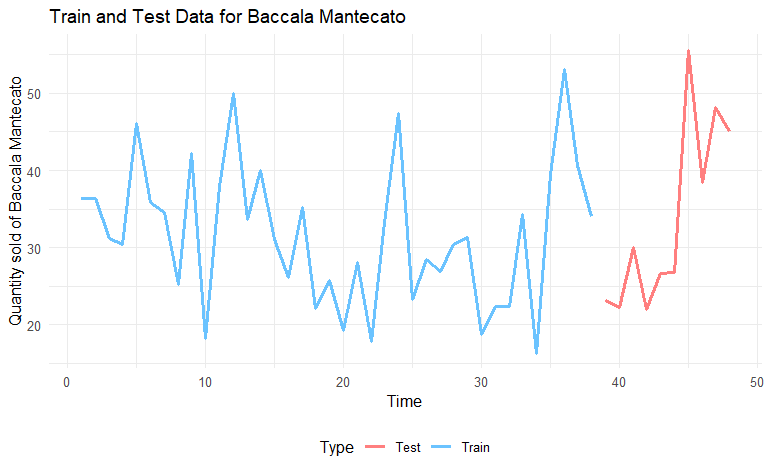
\includegraphics[width=0.5\textwidth]{PlotsBEFD/TRAIN_TEST_MAN.png} 
    \caption{}
    \label{fig:TRAIN_TEST_MAN}
\end{figure}
Baccalà Mantecato (Fig.~\ref{fig:TRAIN_TEST_MAN}): The \textbf{training data} (in blue) exhibits the characteristic variability and seasonal trends observed in the explanatory analysis. The \textbf{testing data} (in red) includes more recent observations, capturing the peak sales period in September.
\begin{figure}[H]
    \centering
    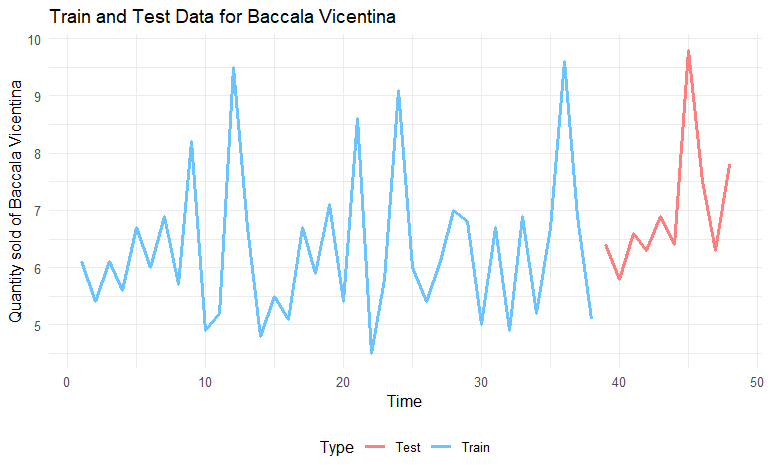
\includegraphics[width=0.5\textwidth]{PlotsBEFD/TRAIN_TEST_VIC.png} 
    \caption{}
    \label{fig:TRAIN_TEST_VIC}
\end{figure}
Baccalà Vicentina (Fig.~\ref{fig:TRAIN_TEST_VIC}): Similarly, the training data reflects the stable yet seasonal nature of sales, while the testing data emphasizes the end-of-year peaks.

Notably, in $2024$, the peak sales for Baccalà occurred in September rather than December, deviating from historical patterns. This anomaly may present challenges for forecasting models, as it represents a shift in seasonal behavior for both the variants.

By implementing this train-test split, the analysis sets the stage for rigorous model development and validation. 


\section{Modelling}
\subsection{Linear Regression Models}
The modeling phase began with the development of \textbf{linear regression models} for both Baccalà Mantecato and Baccalà Vicentina. Each variant required a distinct approach due to their different underlying patterns and relationships with predictor variables.

\subsubsection{Model for Baccalà Mantecato}
For Baccalà Mantecato, the initial model incorporated three key predictors: a \textbf{trend} variable, \textbf{monthly seasonality} indicators, and \textbf{fish consumption} data. The model demonstrated strong explanatory power, with an $R^2$ value of $0.9178$, indicating that approximately $91.78$\% of the variability in Baccalà Mantecato sales could be explained by these predictors.

\begin{figure}[H]
    \centering
    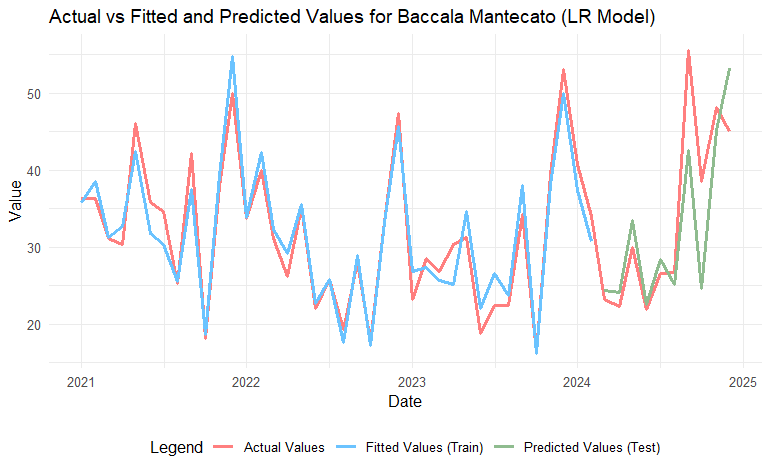
\includegraphics[width=0.5\textwidth]{PlotsBEFD/PRED_LR_MAN.png} 
    \caption{}
    \label{fig:PRED_LR_MAN}
\end{figure}

Analysis of the coefficients revealed several important relationships:

The \textbf{trend} variable showed a positive coefficient of $0.18$, suggesting that, ceteris paribus, Baccalà Mantecato sales increase by $0.18$ units per time period.

\textbf{Fish consumption} demonstrated a strong positive relationship with a coefficient of $7.79$, indicating that for each unit increase in fish consumption, Baccalà Mantecato sales rise by approximately $7.79$ kg. For example, if fish consumption in Italy increases by one unit in October $2021$, the quantity sold in December $2021$ would increase by $7.79$ kg, assuming all other variables remain constant.
The \textbf{monthly} indicators captured significant seasonal effects, with December showing a substantial positive impact and months like February and October displaying negative coefficients relative to the January baseline.

Model selection was performed by systematically removing variables and comparing performance metrics ($AIC$ and adjusted $R^2$) across different specifications:
\begin{itemize}[noitemsep, topsep=0pt]
    \item Model with trend and fish consumption only
    \item Model with trend and monthly seasonality only
    \item Model with monthly seasonality and fish consumption only
    \item Full model with all predictors
\end{itemize}
The comparative analysis confirmed that the \textbf{full model}, incorporating all predictors, provided the \textbf{best fit} according to both $AIC$ and adjusted $R^2$ criteria.

\begin{figure}[H]
    \centering
    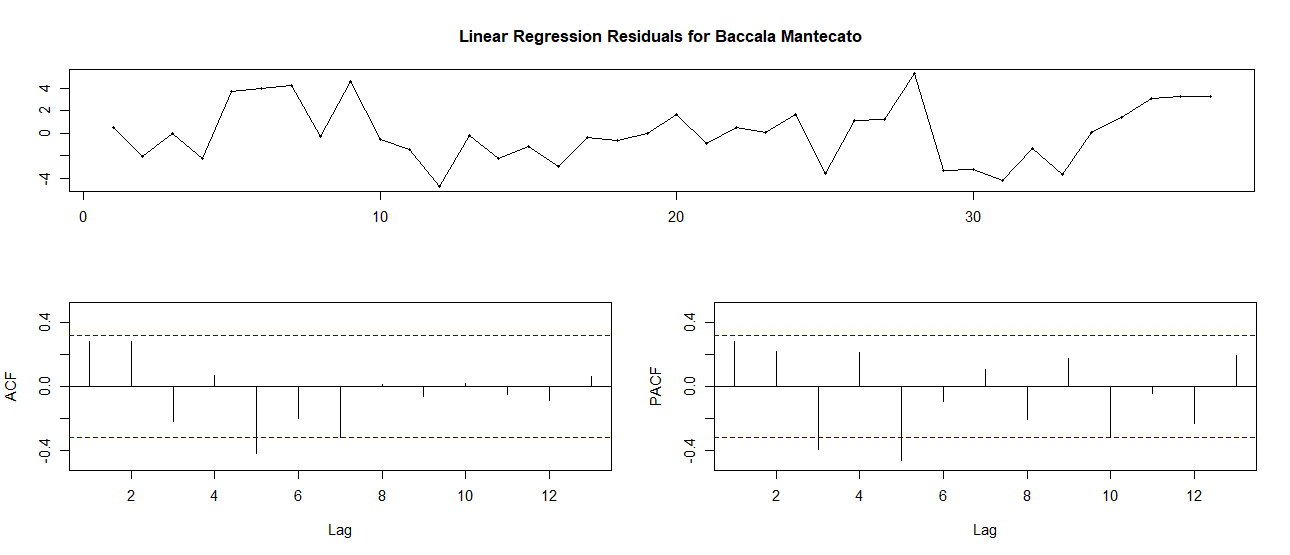
\includegraphics[width=0.5\textwidth]{PlotsBEFD/RES_LR_MAN.png} 
    \caption{}
    \label{fig:RES_LR_MAN}
\end{figure}

Residual analysis (Fig.~\ref{fig:RES_LR_MAN}) revealed patterns and peaks out of the bounds with the \textbf{Durbin-Watson test} that indicates the presence of autocorrelation in the residuals. While we attempted to address this by fitting a linear regression model with ARIMA errors, this approach resulted in \textbf{overfitting}.

\subsubsection{Model for Baccalà Vicentina}
The modeling approach for Baccalà Vicentina followed a similar initial framework but led to different conclusions. The initial full model included the same three predictors: \textbf{trend}, \textbf{monthly seasonality}, and \textbf{fish consumption}. However, the analysis revealed that fish consumption did not significantly contribute to the model's performance.
Through iterative model refinement:

Fish consumption was removed, leading to an improvement in adjusted $R^2$ from $0.8261$ to $0.8305$.
The trend variable was subsequently eliminated due to its high p-value.
The \textbf{final model} retained only \textbf{monthly seasonality} indicators
\begin{figure}[H]
    \centering
    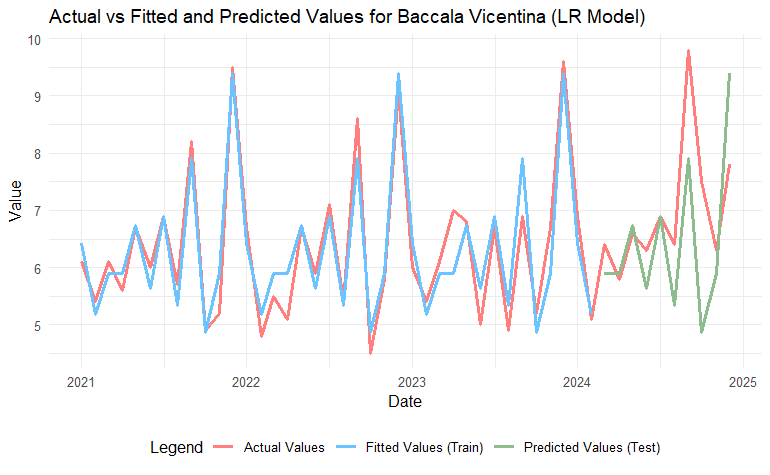
\includegraphics[width=0.5\textwidth]{PlotsBEFD/PRED_LR_VIC.png} 
    \caption{}
    \label{fig:PRED_LR_VIC}
\end{figure}
The simplified model demonstrated strong statistical significance with an \textbf{F-statistic} of $18.21$ (p-value = $1.684e-09$). This suggests that variations in Baccalà Vicentina sales are primarily driven by seasonal effects, without significant influence from trend or fish consumption patterns.
Comparison of model performance metrics confirmed the superiority of the \textbf{seasonality-only} model over the full specification, with improved $AIC$ and adjusted $R^2$ values. 
\newline
The analysis of the historical sales data for Baccalà Vicentina in kilograms reveals notable seasonal effects. December shows a significant positive impact on sales ($+2.975$), likely driven by higher demand during the holiday season. In contrast, October ($-1.558$) and February ($-1.250$) exhibit substantial declines compared to January. Additionally, August records a notable decrease ($-1.092$), potentially reflecting lower summer demand. These results highlight clear seasonal patterns in sales trends.
\newline
Residuals (Fig.~\ref{fig:RES_LR_VIC}) appear randomly scattered:
\begin{figure}[H]
    \centering
    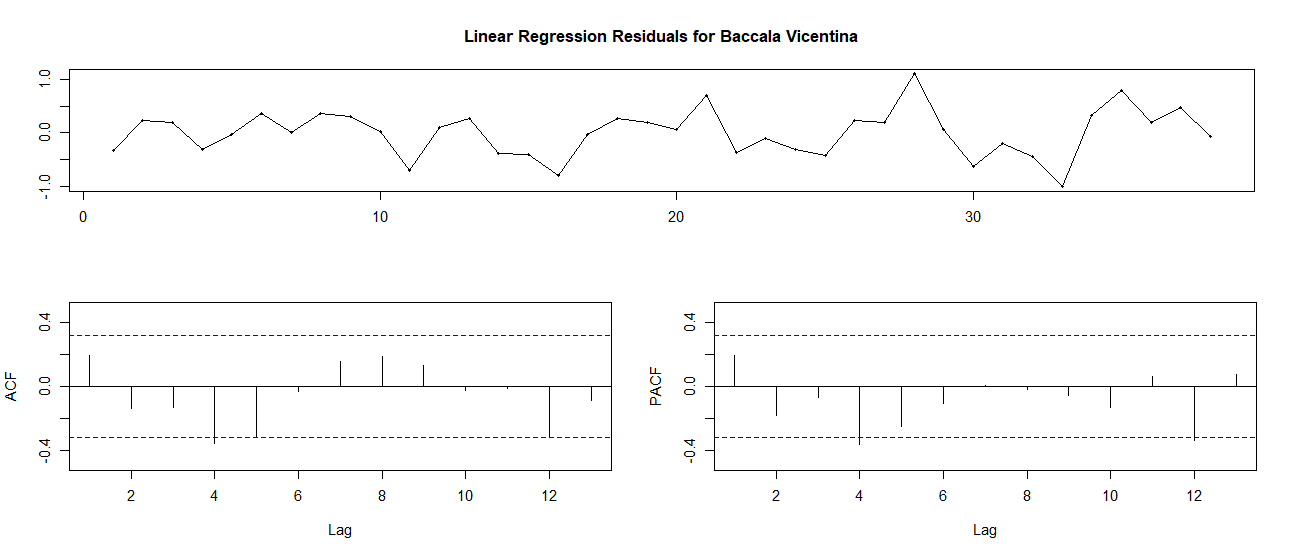
\includegraphics[width=0.5\textwidth]{PlotsBEFD/RES_LR_VIC.png} 
    \caption{}
    \label{fig:RES_LR_VIC}
\end{figure}
This idea is confirmed by the \textbf{Durbin-Watson test} with a p-value ($0.18$) exceeding the $0.05$ significance level.
The distinct modeling outcomes for the two variants highlight the importance of tailored approaches in time series analysis, as similar products may exhibit different underlying patterns and relationships with predictor variables.

\subsection{SARIMA Models}
Following the linear regression analysis, we explored various time series models for both variants of Baccalà. Initial attempts with ARMA and ARIMA models showed poor performance due to the pronounced seasonal patterns in the data. This led us to focus on \textbf{Seasonal Autoregressive Integrated Moving Average} (SARIMA) models, which explicitly account for seasonality in the time series.

\subsubsection{Model for Baccalà Mantecato}
Initial analysis of the Baccalà Mantecato time series confirmed the presence of both trend and seasonal components identified in the regression analysis. After transforming the data into a time series object, we examined the \textbf{autocorrelation} ($ACF$) and \textbf{partial autocorrelation} ($PACF$) functions of the first-differenced series. 

\begin{figure}[H]
    \centering
    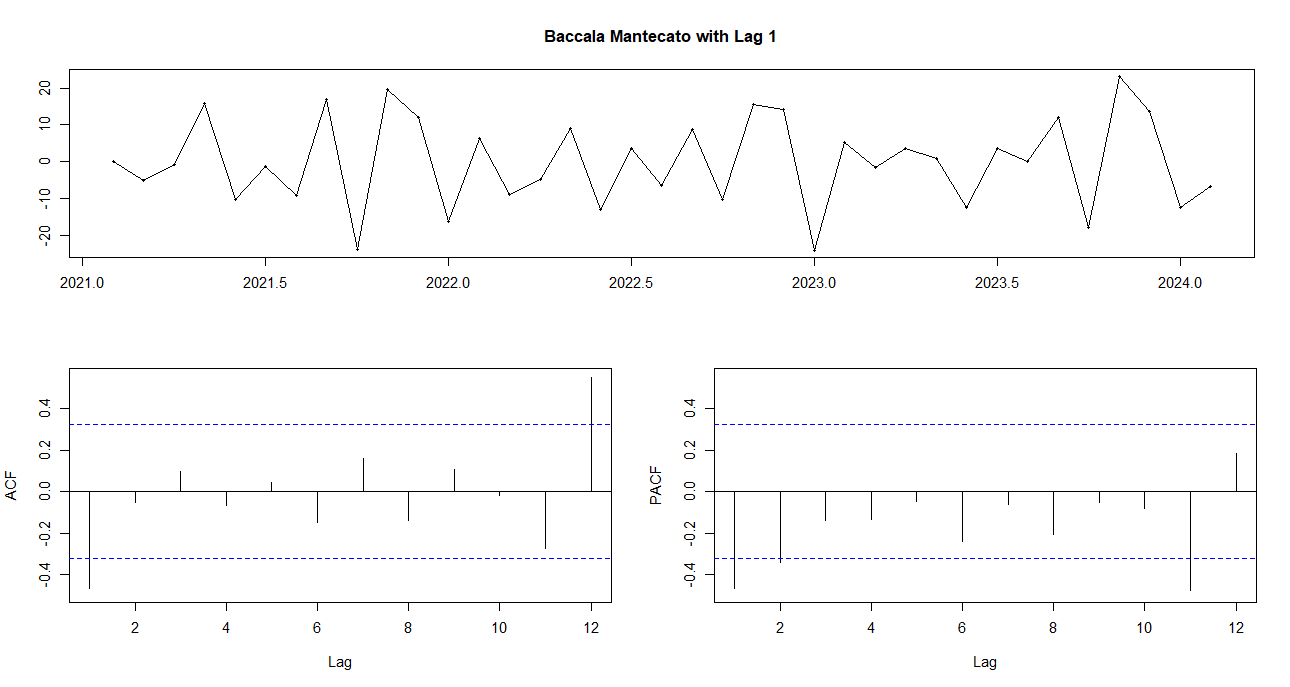
\includegraphics[width=0.5\textwidth]{PlotsBEFD/ACF_MAN_LAG1.png} 
    \caption{}
    \label{fig:ACF_MAN_LAG1}
\end{figure}

Both $ACF$ and $PACF$ plots (Fig.~\ref{fig:ACF_MAN_LAG1}) revealed a distinctive sinusoidal pattern, with values generally within the confidence bands except for a significant spike at lag $12$, strongly suggesting \textbf{annual seasonality in the data}.
To address these patterns, three SARIMA models were evaluated:
\begin{itemize}[noitemsep, topsep=0pt]
    \item \textbf{SARIMA(1,1,0)(0,1,0)[12]}: Includes non-seasonal differencing ($d=1$), one autoregressive term, and seasonal differencing.
    \item \textbf{SARIMA(0,1,1)(0,1,0)[12]}: Incorporates a moving average term instead of an autoregressive term.
    \item \textbf{SARIMA(0,1,0)(0,1,0)[12]}: Uses only differencing components.
\end{itemize}

While the $SARIMA(0,1,1)(0,1,0)[12]$ model showed the lowest $AIC$ value, suggesting better in-sample fit, evaluation on the test set revealed that the simpler $SARIMA(0,1,0)(0,1,0)[12]$ model achieved \textbf{superior out-of-sample performance} with lower \textbf{Mean Squared Error} ($MSE$). This finding highlights the importance of model parsimony and the potential risks of \textbf{overfitting}.
Anyway a $SARIMA(0,1,0)(0,1,0)[12]$ is a model that only applies differences in trend and seasonality, such that the equation becames $(1-B)(1-B^{12})Y_t = \epsilon_t$. 
Once the first difference, \( (1-B)Y_t \), and the seasonal difference, \( (1-B^{12})Y_t \), are applied, the resulting process is governed solely by the random error term \( \epsilon_t \). In other words: the application of the first difference removes the trend component while the application of the seasonal difference removes periodic components associated with annual seasonality (e.g., with periodicity \( s=12 \) for monthly data).
After these transformations, the series essentially becomes white noise: $\epsilon_t \sim WN(0, \sigma^2)$
where \( WN \) represents white noise with zero mean and constant variance \( \sigma^2 \).
Analysis of the residuals for the selected model (Fig.~\ref{fig:RES_ACF_SARIMA_MAN}) showed some patterns that suggest the fit isn't satisfying.
\vspace{-0.4cm}  % reduce vertical space
\begin{figure}[H]
    \centering
    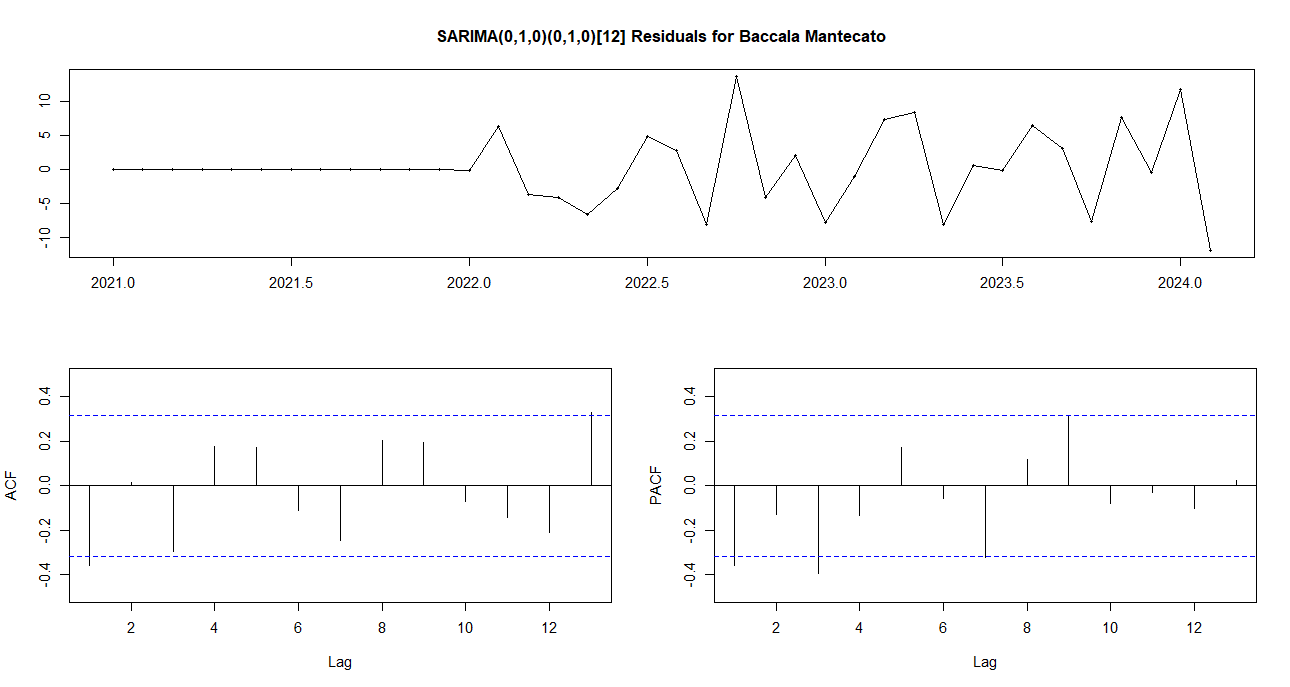
\includegraphics[width=0.5\textwidth]{PlotsBEFD/RES_ACF_SARIMA_MAN.png} 
    \caption{}
    \label{fig:RES_ACF_SARIMA_MAN}
\end{figure}
\vspace{-0.3cm}  % reduce vertical space
However, given its superior test set performance, this model was retained as the final specification for Baccalà Mantecato.

\subsubsection{Model for Baccalà Vicentina}
For Baccalà Vicentina, the time series analysis revealed strong seasonal patterns, with the $ACF$ and $PACF$ functions showing significant spikes at lag $12$, confirming the \textbf{annual seasonality} identified in the regression analysis. 
\begin{figure}[H]
    \centering
    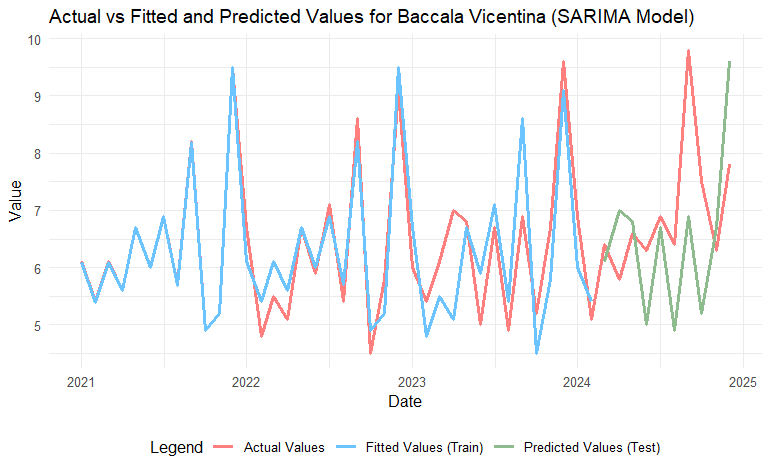
\includegraphics[width=0.5\textwidth]{PlotsBEFD/PRED_SARIMA_VIC.png} 
    \caption{}
    \label{fig:PRED_SARIMA_VIC}
\end{figure}
Unlike Baccalà Mantecato, the series showed less evidence of trend components.
After examining various specifications, a $SARIMA(0,0,0)(0,1,0)[12]$ model was selected.
While models with higher orders of seasonal differencing ($D=2$) produced lower $AIC$ values, they led to higher $MSE$ on the test set, indicating overfitting. The chosen model represents a balance between complexity and predictive accuracy.
\begin{figure}[H]
    \centering
    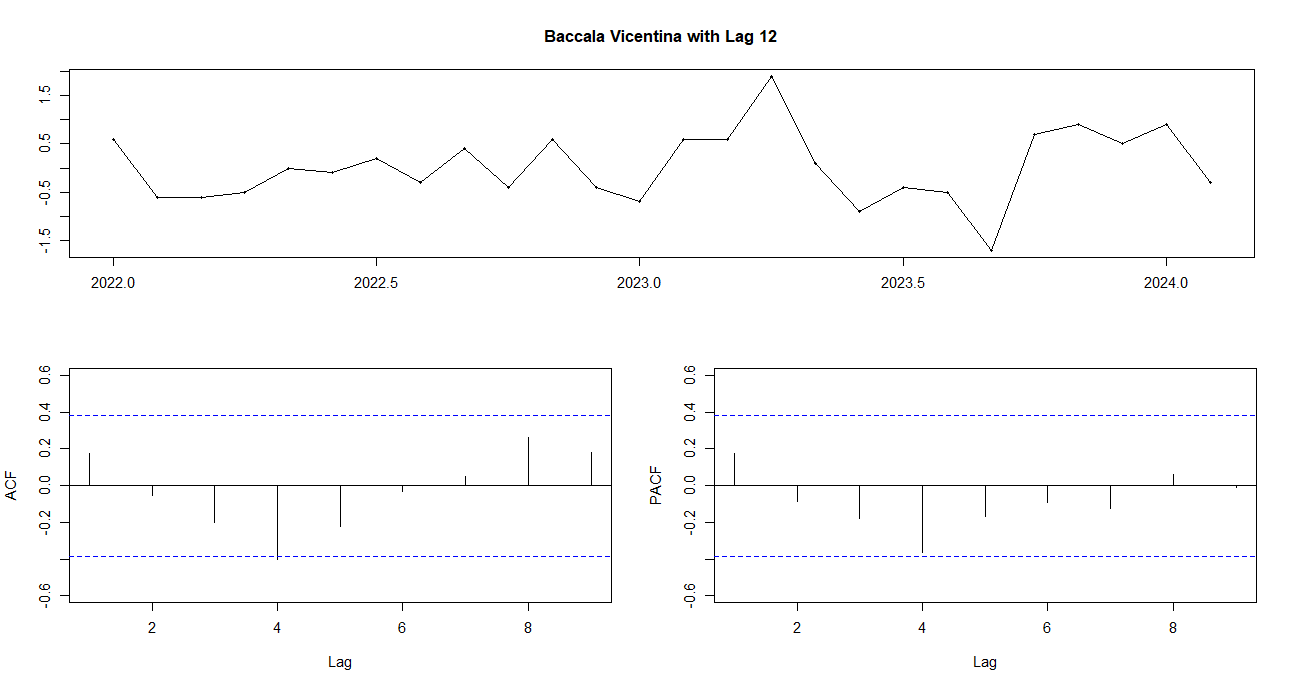
\includegraphics[width=0.5\textwidth]{PlotsBEFD/ACF_VIC_LAG12.png} 
    \caption{}
    \label{fig:ACF_VIC_LAG12}
\end{figure}
The residual analysis (Fig.~\ref{fig:ACF_VIC_LAG12}) of the final model showed some remaining patterns, suggesting that while the model captures the main features of the series, there might be additional structure in the data. However, attempts to incorporate additional ARIMA components did not yield improved performance, supporting the retention of the \textbf{simpler specification}.
These SARIMA models complement the linear regression analysis by explicitly modeling the time series structure of the data, particularly the \textbf{seasonal patterns} that are crucial for both variants of Baccalà. The different specifications required for each variant further emphasize the distinct temporal dynamics of these products, despite their related nature.

\subsection{SARIMAX Models}
To extend our previous analysis with SARIMA models, we decided to include fish consumption as an \textbf{external regressor} (xreg) to evaluate if this addition could improve the models' forecasting performance.

\subsubsection{Model for Baccalà Mantecato}

Initially, we tested ARMAX models, where fish consumption was included as an external regressor.
However, it became clear that the seasonal part of the series had a significant impact on the model's results, as expected from our SARIMA analysis. To address this, we excluded the trend from the xreg variables and instead opted for using differenced time-series.

We then fitted the following models, maintaining the seasonal structure:
\begin{itemize}[noitemsep]
    \item $SARIMAX(1,1,0)(0,1,0)[12]$
    \item $SARIMAX(0,1,1)(0,1,0)[12]$
    \item $SARIMAX(0,1,0)(0,1,0)[12]$
\end{itemize}
The transition from ARMAX to SARIMAX was driven by the need to account for seasonality, which the SARIMAX models handle better through the seasonal component. In the SARIMAX models, we continued to include fish consumption as an external regressor, as it was expected to provide additional explanatory power.

Next, we compared the SARIMA and SARIMAX models using the $AIC$. All SARIMAX models showed an improvement compared to their SARIMA counterparts. However, $AIC$ alone did not capture the complete performance, so we also evaluated the models using $MSE$ on the test set.

The $MSE$ analysis revealed a significant improvement for all three SARIMAX models, reducing the error by approximately $50$\% compared to the corresponding SARIMA models. Considering both $AIC$ and $MSE$, we selected the $SARIMAX(0,1,0)(0,1,0)[12]$ model as the most suitable for forecasting Baccalà Mantecato. Even if the metrics suggest this model, it is not satisfying for the analysis as the counterpart in the SARIMA section, because it is not so far to a simple linear regression on the differenced (with $lag=1$ and $lag=12$) time series.

We then visualized the actual versus predicted values for both SARIMA and SARIMAX models on the test set.
\begin{figure}[h!]
    \centering
    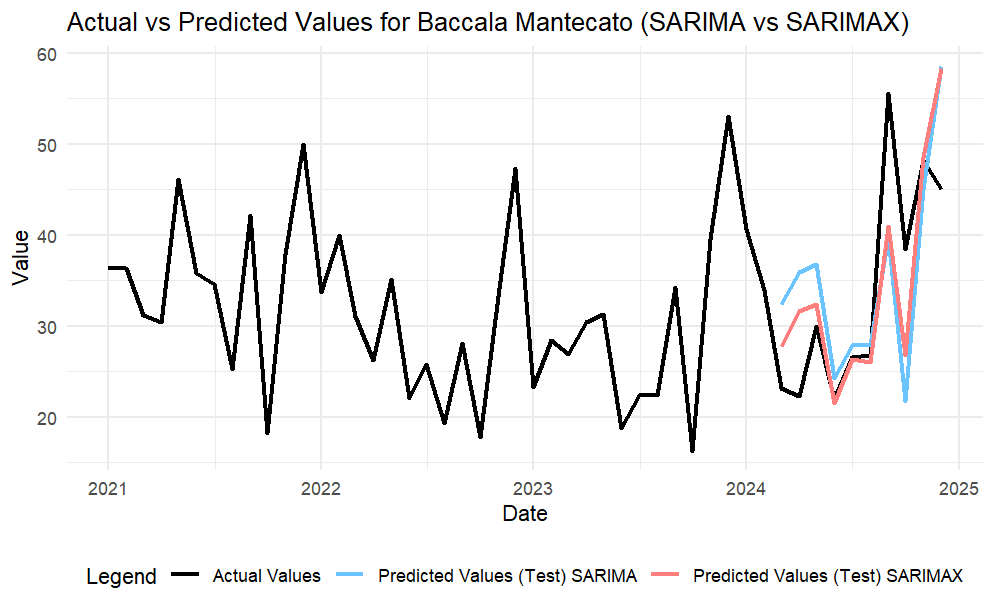
\includegraphics[width=0.5\textwidth]{PlotsBEFD/M_COMPARE_SARIMAX_SARIMA_TEST_PRED.png} 
    \caption{}
    \label{fig:M_COMPARE_SARIMAX_SARIMA_TEST_PRED}
\end{figure}
The plot (Fig.~\ref{fig:M_COMPARE_SARIMAX_SARIMA_TEST_PRED}) highlights the improvement achieved with SARIMAX, confirming the usefulness of including fish consumption as an external regressor in this context.
Residual analysis for the selected SARIMAX model (Fig.~\ref{fig:ACF_SARIMAX_M}) showed some remaining autocorrelation, which suggested the potential need for an autoregressive component. 
\begin{figure}[h!]
    \centering
    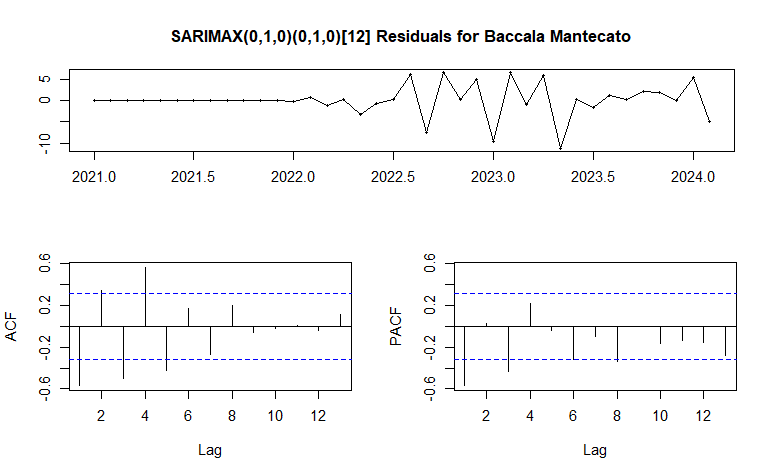
\includegraphics[width=0.5\textwidth]{PlotsBEFD/ACF_SARIMAX_M.png} 
    \caption{}
    \label{fig:ACF_SARIMAX_M}
\end{figure}

Despite this, introducing an autoregressive component led to \textbf{overfitting}, resulting in worse performance on the test set. As a result, we opted to accept the slight loss of information and favored \textbf{generalization} over further model complexity.

Although the $SARIMAX(0,1,0)(0,1,0)[12]$ model shows an improvement compared to its corresponding SARIMA counterpart, we are not satisfied with its performance. With $p$, $q$, $P$, and $Q$ all equal to $0$, the model does not provide a significant advantage over a simple linear regression.



\subsubsection{Model for Baccalà Vicentina}

For Baccalà Vicentina, we followed the same approach as for Baccalà Mantecato, comparing the previously selected $SARIMA(0,0,0)(0,1,0)[12]$ model with a SARIMAX model that incorporated fish consumption as an external regressor:

\begin{itemize}
    \item $SARIMAX(0,0,0)(0,1,0)[12]$
\end{itemize}

We performed the comparison between the SARIMA and SARIMAX models using $AIC$ as the primary metric. The $MSE$ evaluation was also conducted to assess the predictive performance on the test set. Contrary to what we observed for Baccalà Mantecato, the SARIMA model performed slightly better than the SARIMAX model in terms of both $AIC$ and $MSE$. As a result, we decided to discard the SARIMAX model for Baccalà Vicentina and retain the original SARIMA model.

\begin{figure}[h!]
    \centering
    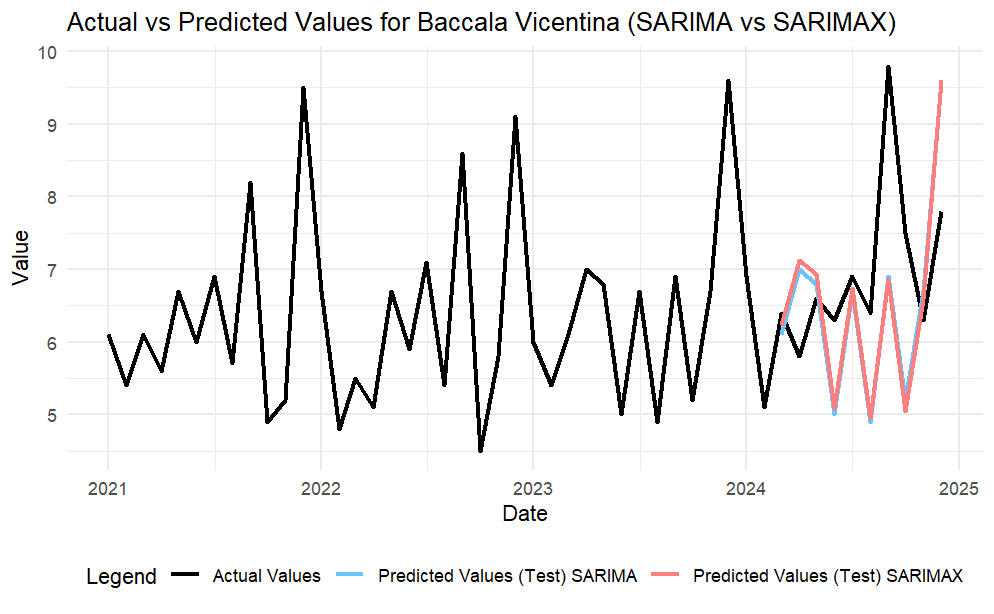
\includegraphics[width=0.5\textwidth]{PlotsBEFD/V_COMPARE_SARIMAX_SARIMA_TEST_PRED.png} 
    \caption{}
    \label{fig:V_COMPARE_SARIMAX_SARIMA_TEST_PRED}
\end{figure}

The plot (Fig.~\ref{fig:V_COMPARE_SARIMAX_SARIMA_TEST_PRED}) shows that both models produced similar performances. Suggesting that adding fish consumption as an external regressor did not enhance the model’s predictive power for this product.

Consequently, we opted to retain the original $SARIMA(0,0,0)(0,1,0)[12]$ model for Baccalà Vicentina, as the inclusion of fish consumption did not provide any tangible benefits.

This comparison illustrates that the effect of including external regressors, such as fish consumption, can vary significantly across product categories. While it improved the predictions for Baccalà Mantecato, it did not offer any benefit for Baccalà Vicentina. These results emphasize the importance of carefully considering the specific characteristics of the time series and the product being analyzed when selecting external factors to include in forecasting models.


\subsection{GAM models}
\subsubsection{Model for Baccalà Mantecato}
In this analysis, we aimed to explore the potential benefits of non-linear models, using \textbf{Generalized Additive Models} (GAM), and compared them to the previously selected Linear Regression model. We started by allowing non-linear relationships between the predictors trend and fish\_cons with the response variable Baccala\_Mantecato.

The plots (Fig.~\ref{fig:GAM_M_LINEARITY}) revealed a possible non-linear relationship. However, further statistical analysis of the model summary indicated that these non-linear relationships were not statistically significant. Specifically, the \textbf{Anova for Nonparametric Effects} showed that the nonparametric \textbf{F-values} for \texttt{trend} and \texttt{fish\_cons} had \textbf{P-values} of $0.1708$ and $0.3461$, respectively. 

\begin{figure}[H]
    \centering
    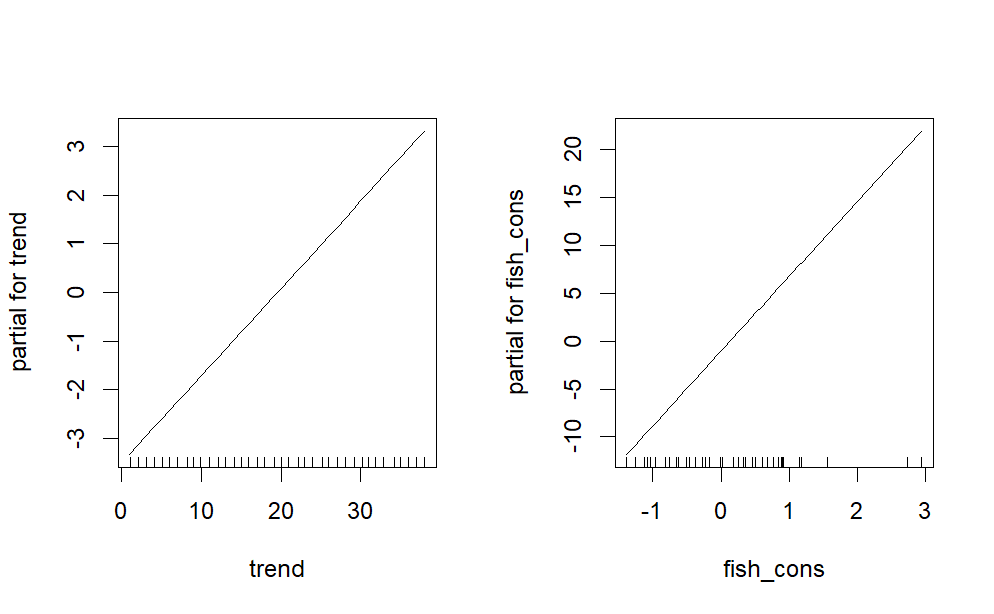
\includegraphics[width=0.5\textwidth]{PlotsBEFD/GAM_M_LINEARITY.png} 
    \caption{}
    \label{fig:GAM_M_LINEARITY}
\end{figure}

These results demonstrated that the GAM model did not provide any significant improvement over the multiple linear regression model. Consequently, for reasons of simplicity, we decided to exclude the GAM model and retain the multiple linear regression model, which better aligns with the data and offers more meaningful and statistically sound results.

\subsubsection{Model for Baccalà Vicentina}
For Baccalà Vicentina, we applied a similar approach to explore potential non-linear relationships between the predictors and the response variable. The visualization of the effects indicated that the behavior of the explanatory variables was consistent with that observed for Baccalà Mantecato, suggesting that non-linear modeling was again unnecessary.

Furthermore, in the section dedicated to linear regression, we had already determined that the best model for Baccalà Vicentina was the reduced model, which included only the \texttt{Month} variable as a predictor. This model was the most effective and parsimonious.

In conclusion, both analyses for Baccalà Mantecato and Baccalà Vicentina indicate that non-linear models such as GAMs do not significantly enhance model performance. Linear models are sufficient for capturing the relationships in the data and provide a more interpretable and statistically sound solution.


\subsection{Prophet model}
For the Prophet model, two distinct models are created for each dish: one with \textbf{logistic growth} and one with \textbf{linear growth}. The choice of model depends on the nature of the data, but both models include yearly seasonality, which is crucial to capturing the seasonal cycles typical of food sales, especially for traditional dishes like Baccalà. The parameter $n.changepoints=5$, that is selected after several tries, trying do avoid overfitting but also to reach a good fit, specifies the number of points in time where the series can experience structural changes. Finally a \textbf{multiplicative seasonality} is selected for both dishes.
\subsubsection{Model for Baccalà Mantecato}
We adapted the model for the Mantecato sales data, and the residuals revealed some issues, particularly highlighted by both the $PACF$ and $ACF$ plots (Fig.~\ref{fig:RES_PROPHET_MAN}), especially with the spike at lag $12$. Despite this, attempts to improve the model by increasing the number of change points or experimenting with different specifications led to a deterioration in performance on the test set.

We also tried to incorporate a model estimated on the residuals using the `$auto.arima$` function, but this did not improve the model's performance. 
\begin{figure}[H]
    \centering
    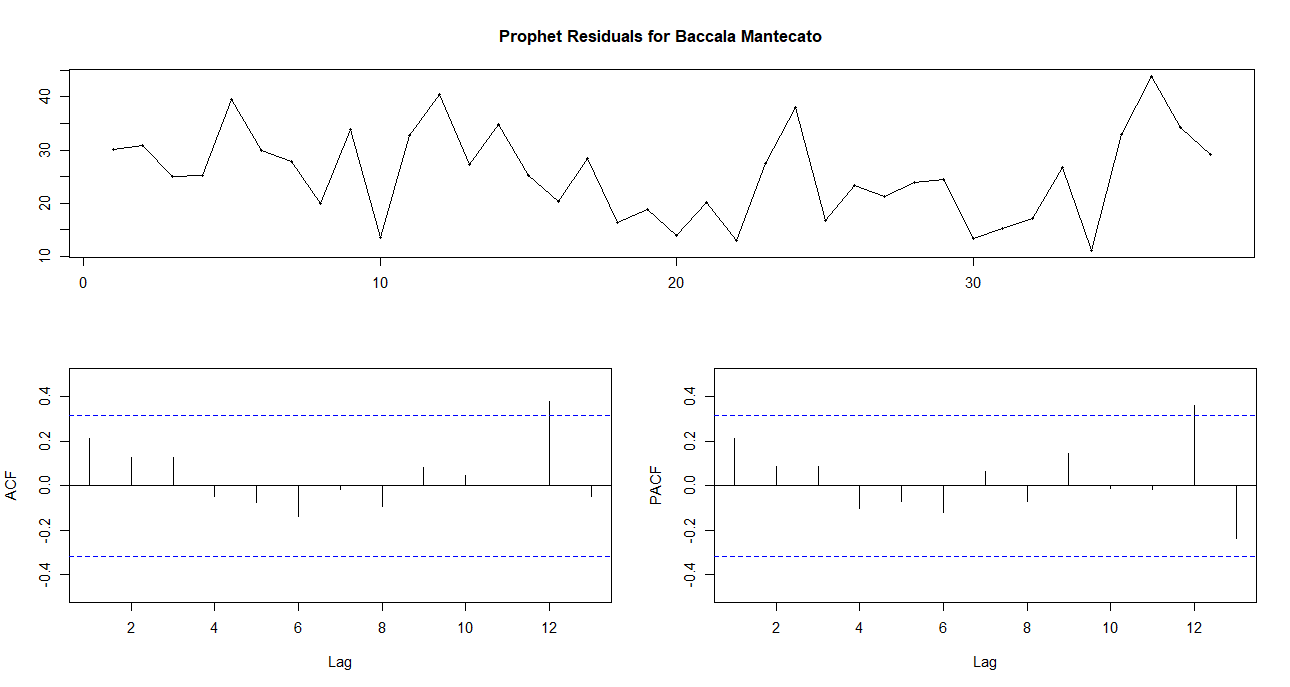
\includegraphics[width=0.5\textwidth]{PlotsBEFD/RES_PROPHET_MAN.png} 
    \caption{}
    \label{fig:RES_PROPHET_MAN}
\end{figure}
Finally, in the graph below (Fig.~\ref{fig:PRED_PROPHET_MAN}), we can observe a good fit to the training data, but the same issues as with the other models are evident on the test set.
\begin{figure}[H]
    \centering
    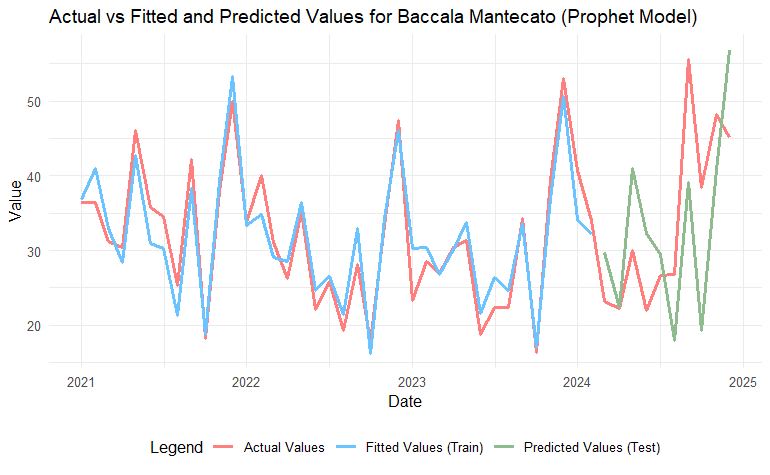
\includegraphics[width=0.5\textwidth]{PlotsBEFD/PRED_PROPHET_MAN.png} 
    \caption{}
    \label{fig:PRED_PROPHET_MAN}
\end{figure}

\subsubsection{Model for Baccalà Vicentina}
The same behavior is observed for Baccalà alla Vicentina, where the residuals (Fig.~\ref{fig:RES_PROPHET_VIC}) show an important spike at lag $12$. 
\begin{figure}[H]
    \centering
    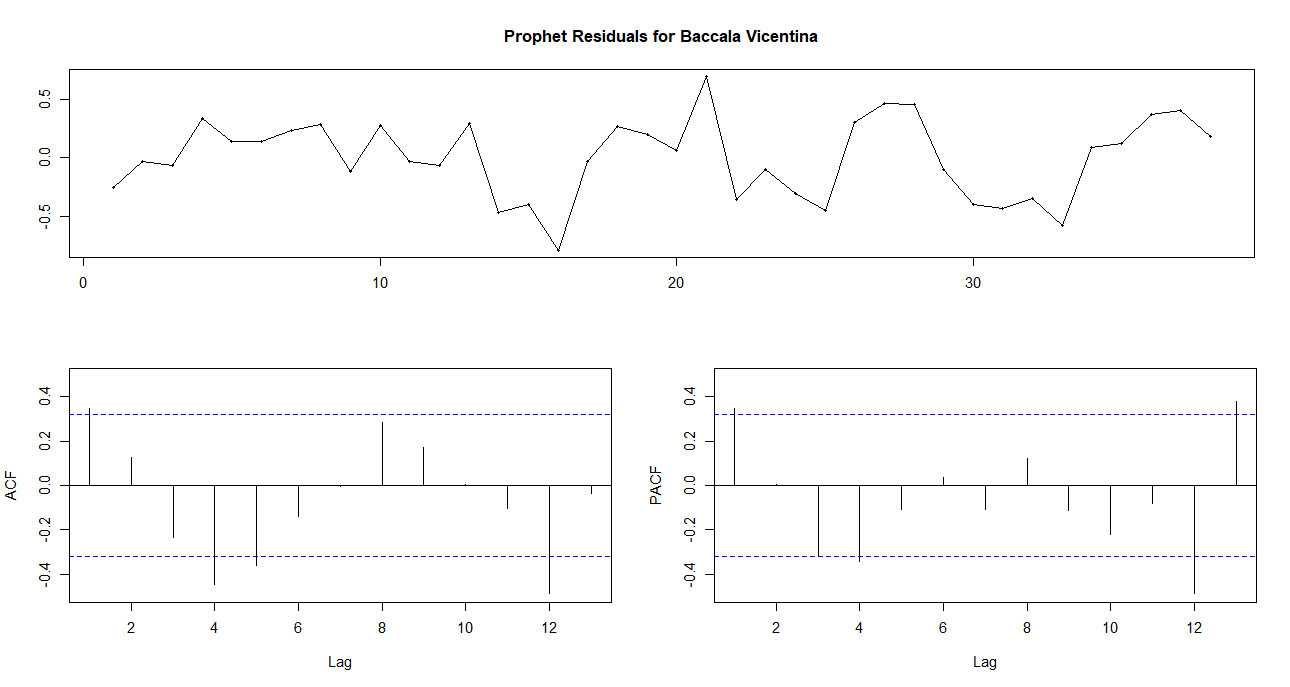
\includegraphics[width=0.5\textwidth]{PlotsBEFD/RES_PROPHET_VIC.png} 
    \caption{}
    \label{fig:RES_PROPHET_VIC}
\end{figure} 
However, we do not want to dwell too much on repeating the same observations, so for completeness, we are including the graph of the actual values versus the predicted ones (Fig.~\ref{fig:PRED_PROPHET_VIC}). 

\begin{figure}[H]
    \centering
    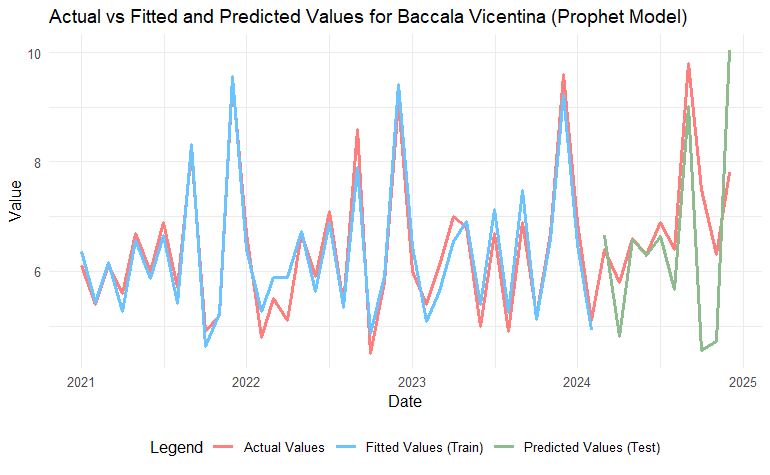
\includegraphics[width=0.5\textwidth]{PlotsBEFD/PRED_PROPHET_VIC.png} 
    \caption{}
    \label{fig:PRED_PROPHET_VIC}
\end{figure}

\subsection{Exponential smoothing Models}
After exploring other approaches, we decided to test \textbf{Exponential Smoothing} (ES) models to analyze and forecast the time series data for Baccalà Mantecato and Baccalà Vicentina. These models are particularly valued for their simplicity and their ability to assign exponentially decreasing weights to past observations, emphasizing the most recent data. They also offer flexibility in handling trend and seasonality, making them ideal for time series with recurring patterns.
For both datasets, we began by testing the classic ETS model (Error, Trend, Seasonality), an approach that automatically selects the optimal configuration based on the data.

\subsubsection{Model for Baccalà Mantecato}
For the Baccalà Mantecato series, the ETS model effectively captured the key dynamics of the data, providing a strong baseline for further analysis. The model demonstrated its ability to adapt to the trends and seasonality present in the series, which were confirmed by both visual and statistical evaluations.
\begin{figure}[h!]
    \centering
    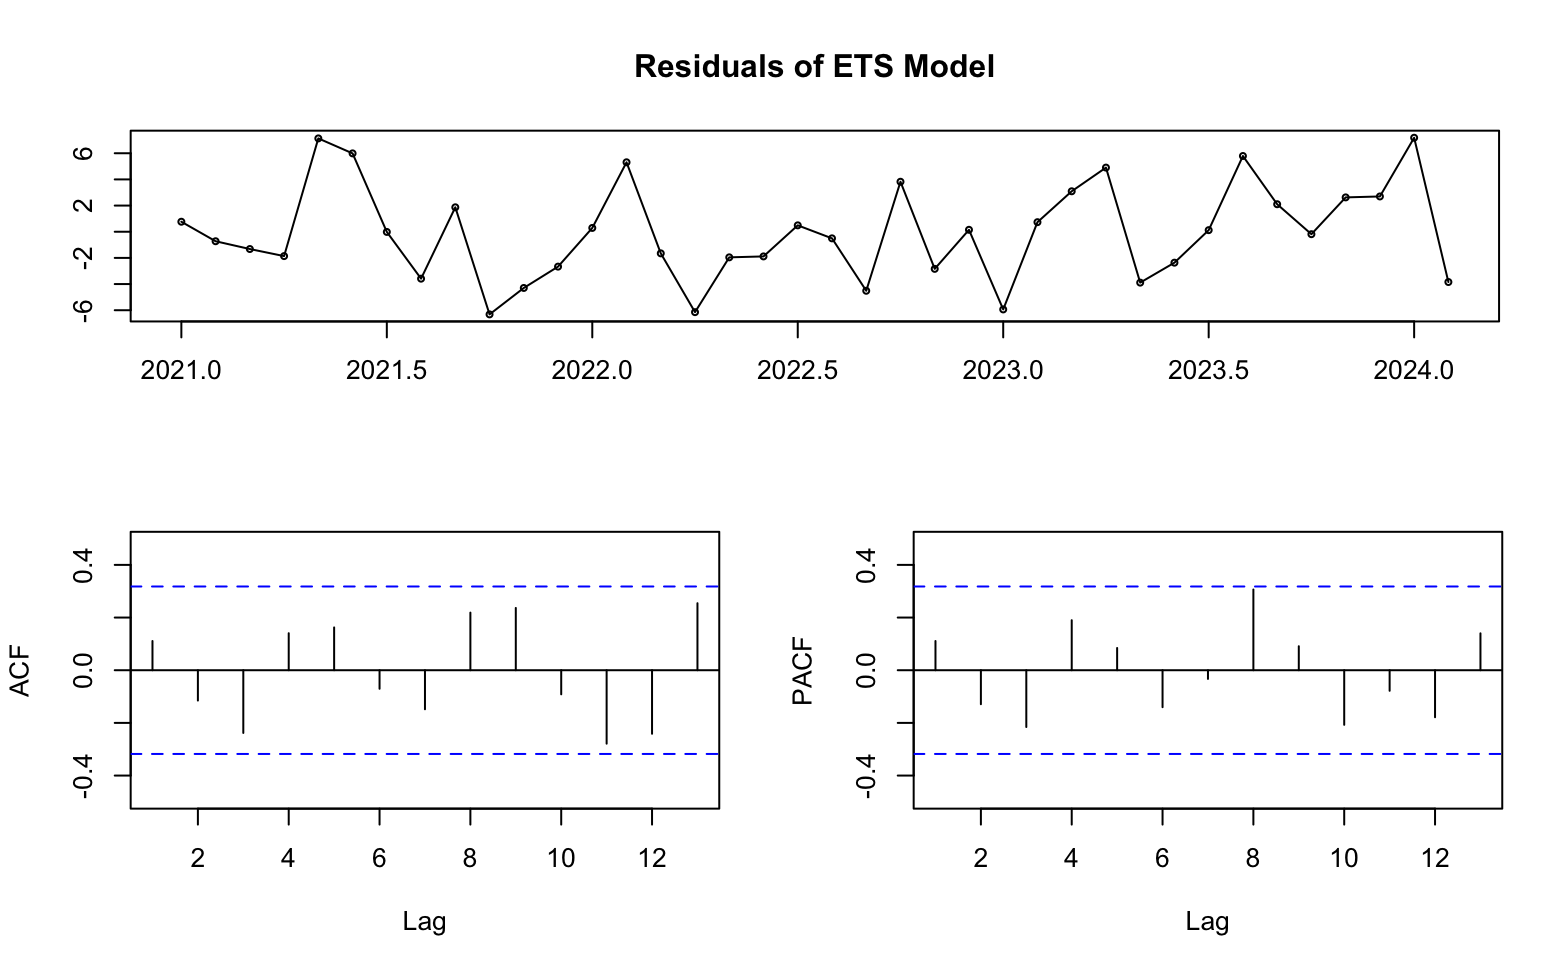
\includegraphics[width=0.5\textwidth]{PlotsBEFD/Residuals_ETS_M.png} 
    \caption{}
    \label{fig:Residuals_ETS_M}
\end{figure}
Residual analysis (Fig.~\ref{fig:Residuals_ETS_M}) revealed that the residuals were randomly distributed around $zero$, with no significant patterns. This indicates that the model successfully accounted for the underlying trends and seasonality, leaving minimal systematic errors. Such behavior is a positive indication of the effectiveness of the ETS model for this time series.
\begin{figure}[h!]
    \centering
    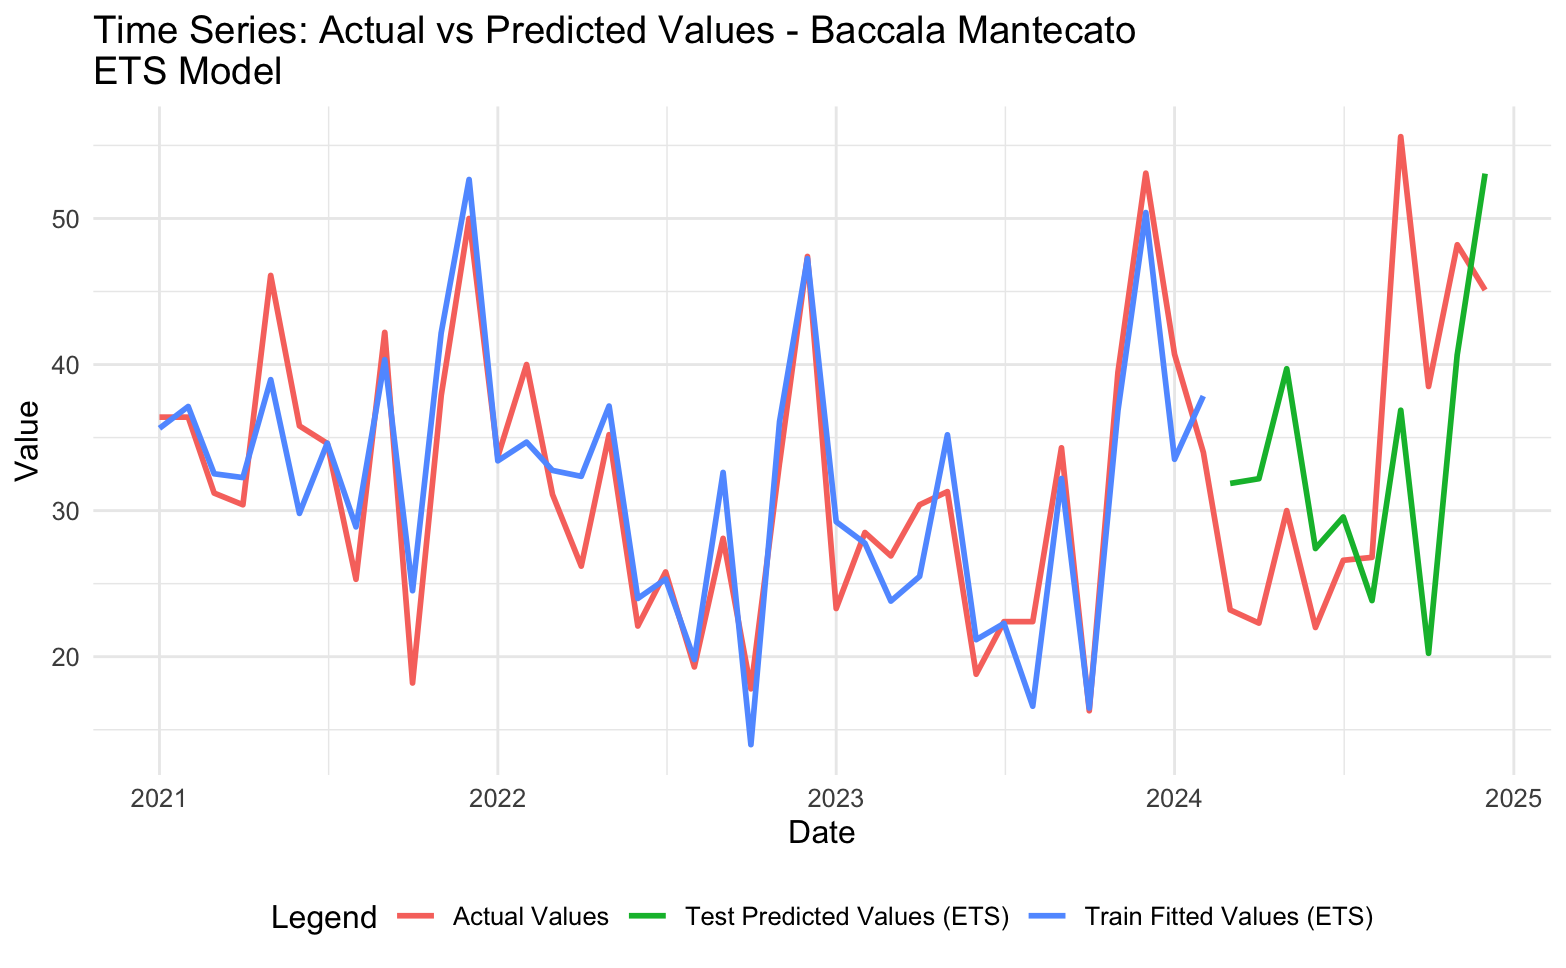
\includegraphics[width=0.5\textwidth]{PlotsBEFD/TS_M_ETS.png} 
    \caption{}
    \label{fig:TS_M_ETS}
\end{figure}

The quality of the forecast was further validated by a visual comparison between the actual and predicted values (Fig.~\ref{fig:TS_M_ETS}). During the training phase, the forecast line closely followed the actual data, reflecting the model's ability to capture key patterns. During testing, the predictions remained near the observed values, with some deviations in the most extreme peaks. This consistency highlights the model's capacity to generalize and handle unseen data sufficiently.

We then explored more specific variants of the ETS model by introducing \textbf{additive} and \textbf{multiplicative} seasonal components through the\textbf{ Holt-Winters} method. Using the additive approach resulted in slightly worse outcomes compared to the standard ETS model, with increases in both the $MSE$ and the $AIC$. These metrics indicated that the added complexity of the additive approach did not yield significant benefits. The multiplicative approach for seasonality provided even less satisfactory results, with higher errors and increased complexity, confirming that the original ETS model was the best option for this series as we can see from (Tab.~\ref{table:model_comparison_man}).

\begin{table}[h!]
\centering
\begin{tabular}{|l|r|r|}
\hline
\textbf{Model} & \textbf{MSE} & \textbf{AIC} \\
\hline
ETS & 111.7995 & 266.4093 \\
Holt-Winters Additive & 114.8030 & 274.4056 \\
Holt-Winters Multiplicative & 177.2098 & 274.7737 \\
\hline
\end{tabular}
\caption{Comparison of Models based on MSE and AIC | Baccalà Mantecato}
\label{table:model_comparison_man}
\end{table}

\subsubsection{Model for Baccalà Vicentina}
Turning to the Baccalà Vicentina series, the behavior of the models was similar, but presented an interesting difference. Once again, the ETS model produced strong initial results, with a low $MSE$ and a favorable $AIC$. However, incorporating \textbf{multiplicative seasonality} through \textbf{Holt-Winters} led to a slight reduction in $MSE$, albeit at the cost of a higher $AIC$ (Tab.~\ref{table:model_comparison_vic}).

\begin{table}[h!]
\centering
\begin{tabular}{|l|r|r|}
\hline
\textbf{Model} & \textbf{MSE} & \textbf{AIC} \\
\hline
ETS & 1.475781 & 105.6035 \\
Holt-Winters Additive & 1.512441 & 111.4078 \\
Holt-Winters Multiplicative & 1.434768 & 109.9921 \\
\hline
\end{tabular}
\caption{Comparison of Models based on MSE and AIC | Baccalà Vicentina}
\label{table:model_comparison_vic}
\end{table}

This trade-off between forecast accuracy and model complexity led us to select the \textbf{multiplicative seasonal model} as the most suitable for this series. While the increase in $AIC$ reflected higher complexity, our primary goal of \textbf{minimizing forecast errors} justified this choice.
\begin{figure}[h!]
    \centering
    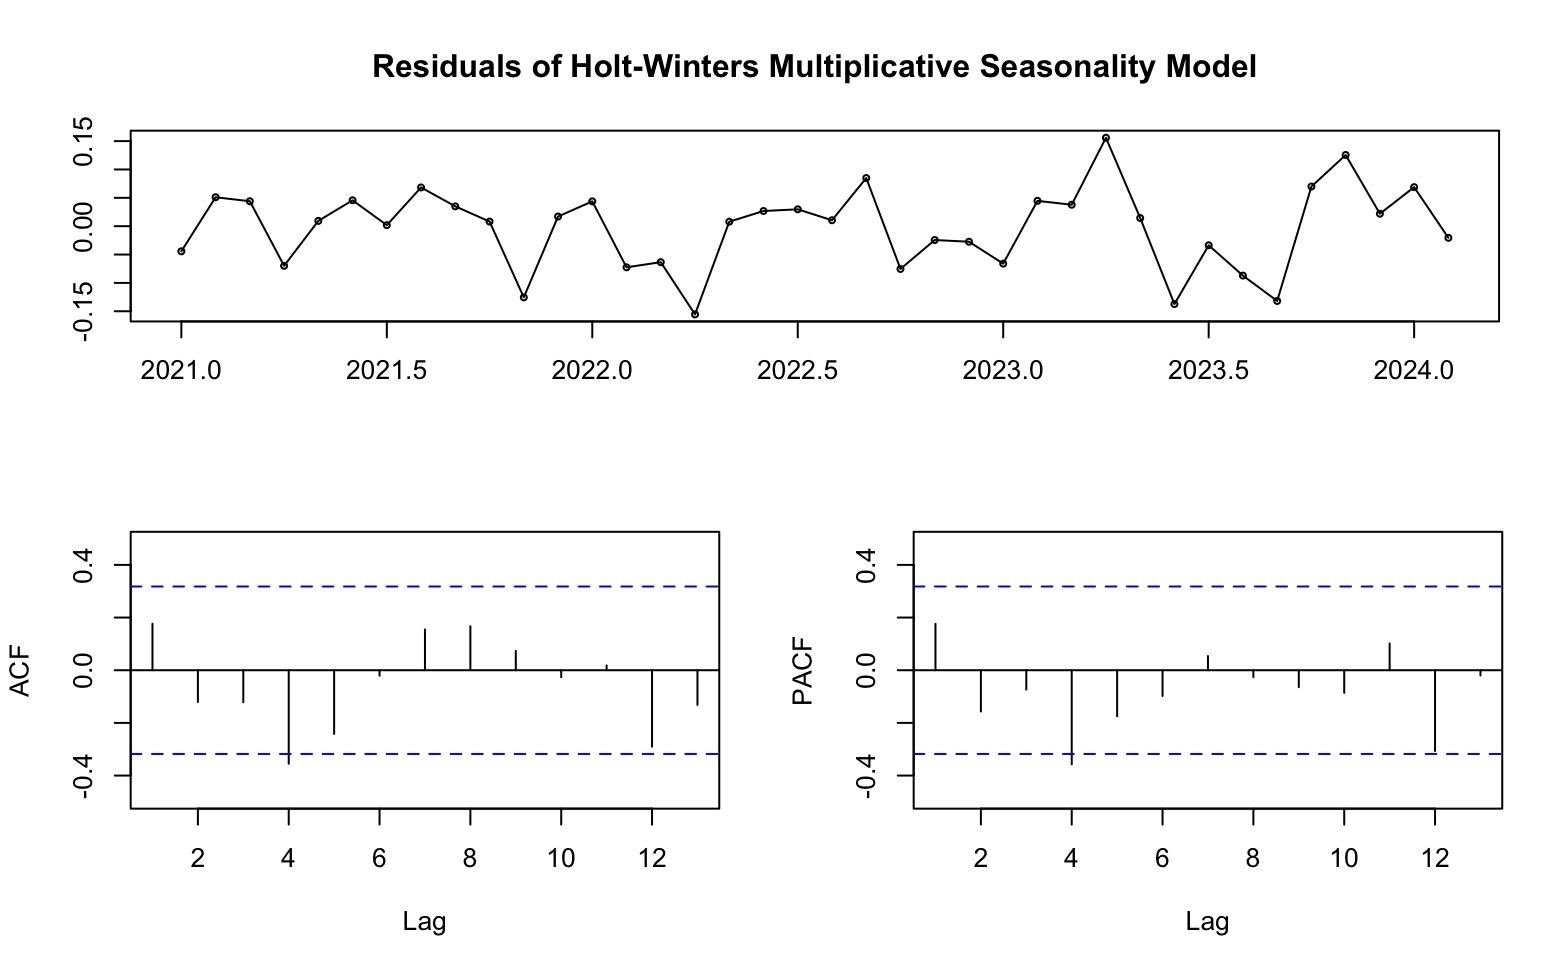
\includegraphics[width=0.5\textwidth]{PlotsBEFD/Residuals_HWM_V.png} 
    \caption{}
    \label{fig:Residuals_HWM_V}
\end{figure}
Residual analysis (Fig.~\ref{fig:Residuals_HWM_V}) confirmed that the selected models effectively captured the main characteristics of the time series. The residuals were randomly distributed around $zero$, showing no repeated patterns and indicating no systematic errors. 

The absence of significant spikes in the residuals' $ACF$ and $PACF$ plots further reinforced this conclusion. This is a strong indication that the chosen model is robust and reliable for forecasting purposes.

\begin{figure}[h!]
    \centering
    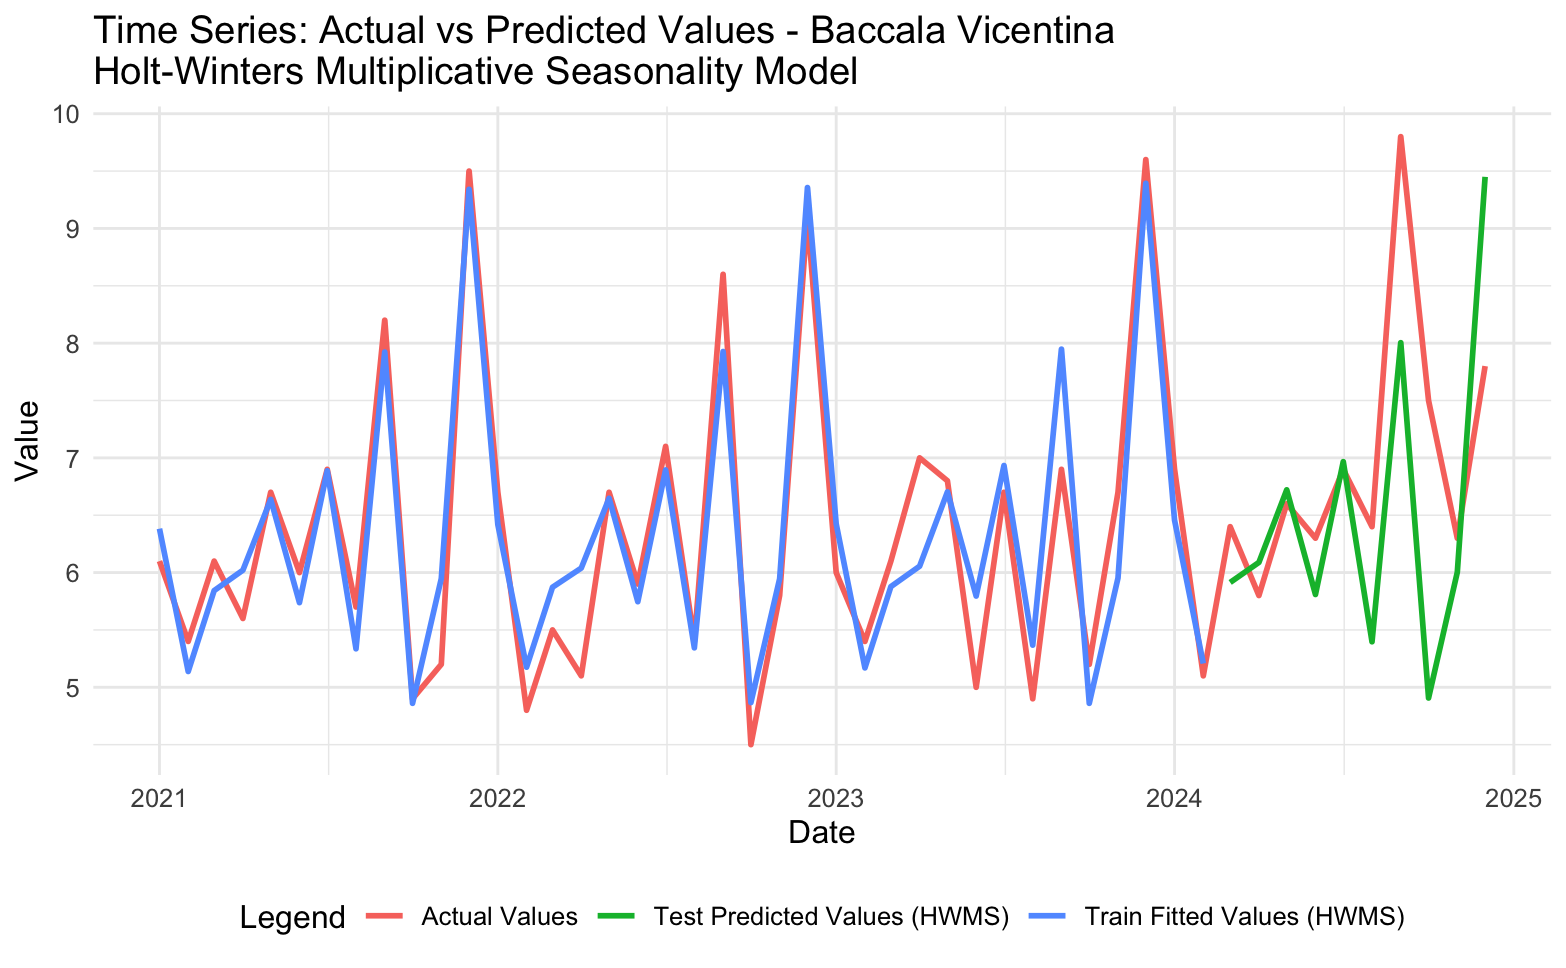
\includegraphics[width=0.5\textwidth]{PlotsBEFD/TS_HWM_V.png} 
    \caption{}
    \label{fig:TS_HWM_V}
\end{figure}

Finally, the forecast plot (Fig.~\ref{fig:TS_HWM_V}) clearly illustrated the models' ability to follow the trends and seasonality in the training phase. In the \textbf{test phase}, instead, the green line representing the predicted values shows a good alignment with the actual values, maintaining the seasonal structure. Some underestimations occur during sharp spikes in the data, but overall the model provides \textbf{reliable forecasts}.

\section{Conclusions}

In this last section we are going to compare the results of the different models on the training and test sets. To compare and properly discuss these results we created a table (Tab.~\ref{table:model_comparison_inverted}) with the $MSE$ values for each model on the training and test sets.

\begin{table}[H]
\centering
\resizebox{1\linewidth}{!}{%
\begin{tabular}{|l|l|l|l|l|}
\hline
\textbf{Model} & \textbf{Train\_M} & \textbf{Train\_V} & \textbf{Test\_M} & \textbf{Test\_V} \\
\hline
\textbf{LR} & 6.7755 & 0.1879 & 45.5953 & 1.5124 \\
\textbf{SARIMA} & 29.7579 & 0.3605 & 104.5050 & 2.2650 \\
\textbf{Prophet} & 9.2290 & 0.1130 & 119.0730 & 1.8423 \\
\textbf{SARIMAX} & 14.2973 & 0.3683 & 64.0557 & 2.3494 \\
\textbf{ETS} & 13.2462 & 0.1936 & 111.7995 & 1.4348 \\
\hline
\end{tabular}
}
\caption{Performance metrics for different models (MSE)}
\label{table:model_comparison_inverted}
\end{table}

From the table \ref{table:model_comparison_inverted}, several insights can be drawn regarding the performance of the models.

The results show that Linear Regression provided the best performance, achieving the lowest \textbf{mean squared error} on the test set. However, at the same time, the discrepancy between the results obtained on the training set and those on the test set suggests a possible case of \textbf{overfitting}. This observation applies to all analyzed models and has been the subject of numerous investigations to understand the reasons behind it, which we aim to address in future analyses. % when we are going to address this future analysis?

The best alternative to Linear Regression, in our assessment, is the SARIMAX model. By incorporating the effect of the exogenous variable, SARIMAX outperforms models that only account for seasonality and trend.

An interesting observation regarding the \textbf{test set performance}, as previously mentioned, is the significant discrepancy between training and test results. Analyzing the historical series, we observed that the peak for $2024$ occurred in September, whereas in previous years, it consistently occurred in December. However, all models predicted the peak for December $2024$, adhering to historical trends that were not followed in the most recent year. This anomaly remains unexplained.

A practical limitation of the Linear Regression model is its dependence on the exogenous variable ($fish\_cons$), which is necessary for making predictions. For instance, to forecast the value for January $2025$, the $fish\_cons$ data for November $2024$ is required. Since this data is sourced online, there is no guarantee it will be updated frequently enough, potentially compromising the timeliness of the forecasts. This limitation also applies to SARIMAX, which is why a model like SARIMA could be considered as an alternative.

For Baccalà Vicentina, the issues are similar: the test set is not representative of the training set, and evaluating the models' performance on the test set distorts the results. In this case, the best-performing model on the training set is \textbf{Prophet}, but it is outperformed by the \textbf{Holt-Winters Multiplicative model} on the test set. This result suggests, as evidenced by the p-values in the regression model, that the relationship with the $fish\_cons$ variable is not statistically significant.

Although the results for Baccalà Vicentina initially appear better than those for Baccalà Mantecato, the scale of the data must be considered. The quantities in kilograms sold for Baccalà Vicentina are roughly between $1/4$ and $1/3$ of those for Baccalà Mantecato. During our analyses, we tested additional models, for both the response variables, such as introducing non-linear trends (look at the code), but, as expected, none of these produced significant improvements for our objective.

Overall, the analysis demonstrates that certain models are preferable to others and that the most complex model is not always the best-performing one. For example, adding transformations of the trend and $fish\_cons$ variables in the code did not yield better results. However, due to the ambiguous behavior of the time series in the test set and the lack of a clear explanation for it, we cannot be certain that using the model for business purposes will be valid and achieve the same level of accuracy observed in the training set.

This analysis was both challenging and insightful. 
On one hand, the quality of the data proved to be inadequate due to the limited time series (only $36$ observations) and a test set that, in our opinion, was not representative of the training set. This discrepancy distorted our evaluation of the models’ performance. 
On the other hand, it was stimulating to address a real-world problem and to observe how two seemingly similar products—Baccalà Mantecato and Baccalà Vicentina—exhibited markedly different behaviors.

Data collection required significant effort, starting with an initial meeting to present our proposal and understand the client’s needs, followed by a second meeting to manually extract and transcribe data from invoices. Additionally, sourcing external data presented its own set of challenges. 
We explored websites such as \textbf{ISTAT}, \textbf{Eurostat}, and \textbf{EUMOFA}, but many attempts turned out to be fruitless. 
Nonetheless, we successfully identified a variable—salmon quantities—that appears to correlate with Baccalà trends, even if this might be a coincidence.

Our mission was to provide an accurate yet interpretable model to explain our findings to \textit{Arte Culinaria da Jhonny}. 
We believe we achieved this goal, especially for Baccalà Mantecato, which is also the establishment’s flagship product (see the interpretation of linear regression coefficients for details).

A key recommendation we made to the business is to maintain an active collaboration. 
This would allow for the collection of a more extensive time series in the future and facilitate the identification of additional factors influencing the target variables. 
Incorporating these factors into the model could enhance its performance and provide actionable insights for the business.
\end{document}
